% 2 pages -- Aaron
%\subsection{Overview}
 % Describe the system - create an image
%\subsection{Static Analysis}
%\subsection{Dynamic Analysis}
%\subsection{Database Schema}
For the automated analysis, rather than exclusively developing our own tools, we relied as much as possible on existing production quality tools and environments.
%TODO -- you need to explain what information are you extracting from the compiler --- you need to mention that you are extracting the Abstract Syntax Tree, and what other analysis and that you are leverging from gfortran intermediate representation data structures, where you are making a bridge from the intermediate program representation to SQL.
%AS: cite Allinea MAP
Our method extracts data about code directly from a production compiler \ac{GCC}, initially with an exclusive focus on Fortran, and optionally uses a scalable performance analysis tool (Allinea MAP) to obtain information on run-time characteristics.
The optional dynamic analysis is run separately by the user to collect periodic samples of where the application is spending time.
These two sources of information are inserted into tables in an \acs{SQL} database, which then allows for queries to be run using one or both sources of data to gain insight into the code's execution.
An illustration of the this flow can be seen in Figure~\ref{fig:design}.
These steps will be addressed separately in the following subsections.
While we include components of a dynamic analysis in this way, we primarily emphasise the use of static information, with the dynamic analysis mostly used to narrow the focus more specifically on regions of particular interest and supplement the functional data (e.g. of routines invocations, loop trip counts, etc) obtained from the compiler with additional non-functional data (e.g. hardware counter information) obtained from the performance tool.

\begin{figure}
\begin{center}
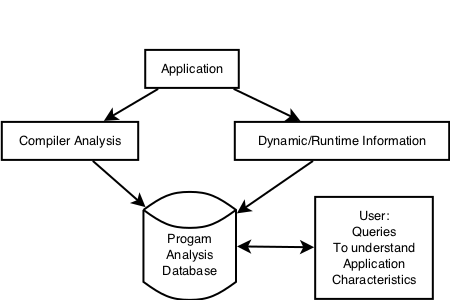
\includegraphics[width=0.4\textwidth]{images/design.png}
\end{center}
\caption{Tool Design}
\label{fig:design}
\end{figure}

The result of this analysis is two-fold in that both system administrators and support staff as well as users (with optional supplementary run-time data) are able to get answers to questions about applications relevant to their own needs and interests.
We will demonstrate a few examples of this investigative ability in Section~\ref{sec:casestudy}.

%The desired result of this analysis is to achieve similar results to what the manual tweaking of our previous work found so that it can more realistically and scalably be applied to larger and more complex applications.
%To this end, we will compare the results from our previous work to what we achieved with our new tools to determine how well they are able to match up.
%We will then perform a reverse validation by applying the same analysis to a different and larger application that was not part of our previous work, modify the memory placement for the reported hotspots, and see how well the actual results fall in line with the expected results.
%This will be described in more detail in Section~\ref{sec:results}.
\subsection{Static Analysis}
%TODO: particular spec/features of fortran?
For the static analysis, we relied on the \ac{GCC} for its support of Fortran.
%This seems to be not very interesting for the paper -- this is just mechanics (Loading a module)
Using its plugin \acs{API}, we created a module to be loaded and run after the compiler finishes parsing the code.
%TODO: poly
%Additionally, it also registers a pass to be run while it's generating its GIMPLE \ac{IR} in order to get additional analysis information from the lower stages of the compiler.
The plugin runs through all the relevant data structures in the \ac{AST} representing the code to queue the data, then proceeds to dump them all at once in bulk transactions.
For the database, we used PostgreSQL for some of its advanced query support.
\subsubsection{Dumping the Static Data}
We did not attempt to create our own schema to represent the code, as it would not immediately be necessary due to the tables not being intended as a user-facing interface and our current focus on Fortran not requiring a new language agnostic schema.
%TODO: no possessive acronyms... :'(
Instead, we simply dumped out \ac{GCC}'s internal data structures such that each data structure was a table, and each member of the data structure was a column.
We currently extract information from 160 \acs{GCC} data structures (tables) consisting of 1014 fields (columns).
Eventually, once enough queries have been made for users, it may then be possible to reduce the level of information down if there is a great enough difference between what is captured and what is actually used, but that is left for future work.
%TODO: technically not all tables...mention enums?
Common to all tables are two columns for the pointer to the data structure in memory during compilation, and a build ID unique to each compilation unit.
%TODO: necessary to very briefly explain primary/foreign keys, etc, or are they sufficiently self-describing?
Together, these two fields form the table's composite primary key to uniquely identify each record in the database.
Furthermore, this also allows us to dump all data in the most straightforward of manners - primitive types get dumped as their corresponding \acs{SQL} data type, and pointers to other objects as the raw value of those pointers.

This part of the data can be obtained automatically and without the direct involvement of the user, using the same methods used by XALT \cite{7081224}.
That is, a wrapper can be made for \ac{GCC} to intercept compilation and make it use the necessary plugin, and dump the data either to files, a system log, or directly to the database.
In addition to the primary data about the code itself, XALT is able to insert a unique identifier into each linked application.
An additional relation between this link ID and the compilation unit build IDs used for each of the files being linked must be made so that when applications are run, they can be tied back to each of the particular compilations and associated data, which we also need here for connecting the dynamic data at a later stage.
\subsubsection{Querying the Static Database}
Due to the way we identify records and store object references, we are able to use any columns representing pointers as foreign keys with which to join connected tables in the database.
One of the most important things we need the database to do for us is associate each code line with file lines.
A lot of our focus on the analysis is dependent on lines of code, so our queries were constructed so as to be able to clearly relate what file and line numbers are involved in an operation.

While a full overview of the schema is best left to the compiler's documentation \cite{gcc-docs}, we will briefly detail a few key structures and fields here to give an idea on what kind of information can be queried.
First, we start with what is referred to as a namespace (internally, \texttt{gfc\_namespace}), which describes the contents of procedures, modules, interfaces, and block constructs.
Starting from the root, each \texttt{gfc\_namespace} contains references to any contained namespaces, a reference to that namespace's symbol tree (\texttt{gfc\_symtree}), and a reference to the first code statement (\texttt{gfc\_code} when applicable.
A code statement is used to represent each individual operation in the code, including assignment, \acs{I/O} operations, conditionals, loops, and function calls.
Each \texttt{gfc\_code} contains fields for the operation type (\texttt{gfc\_exec\_op}), the location it exists in the code, its symbol tree, its contained expressions (\texttt{gfc\_expr}), references to the next statement (if there is one) and the first statement in the contained block of code it starts (e.g. as in the case of loops), and any supplementary information specific to particular operation types such as iterators, or in the case of OpenMP statements, a reference to another table (\texttt{gfc\_omp\_clauses} containing information on the clauses.
Expressions are actually represented as expression trees, where each node contains the type of expression (e.g. constants, variables, arithmetic expressions), its location in the code, its symbol tree, and references to its child expressions (if it isn't a leaf node).
Finally, each symbol (\texttt{gfc\_symbol}) in a symbol tree contains the symbol's name, type, module/scope, its declaration location, and attributes.

We are able to use the data in these tables to perform the reference counting needed in section~\ref{sec:casestudy}.
At a high level, we go through each statement for each namespace and look up on which files and lines they occur, traverse the expression trees for those statements, filter for expressions containing references to variables, then finally check the symbol table to determine which particular variables are being referenced.
We can optionally enhance this further, such as by selecting only variables within particular functions of interest, variables of a particular type, variables being assigned to, and/or variables within OpenMP regions.
Finally, we can combine the results with that of the dynamic analysis detailed in section~\ref{sec:dynamic} so as to know how many times each line was seen in actual execution.
In this way, we are then able construct queries to tally the total number of references observed for every variable across any subset of lines.

This high level overview of a reference counting query hides a number of the difficulties in actually constructing such queries, however, which exist due to the fact that \acs{GCC}'s internal data layout does not perfectly translate to many of the kinds of queries we would like to perform.
While a full explanation of all of these would be excessive for our purposes here, we will briefly describe a couple such issues to aid in closing the gap for future query examples.
One of the biggest of these is actually the process of matching up expressions within the code to line numbers and both statements and expressions to namespaces for selecting by function name.
The reason for this lies in the fact that this information ultimately resides in higher levels - for instance, a \texttt{gfc\_namespace} references a \texttt{gfc\_symbol} containing the name for the namespace, but none of the \texttt{gfc\_code} statements connected to the namespace have any reference back to it.
Additionally, statements can span across multiple lines in files, but we want to bundle them up and count them as a unit, especially since a profiler will most likely provide just one of them, even though we know that all expressions within a statement will get executed together.
As such, we created new tables for these structures to provide additional columns with the data we desired, which we had to populate by traversing and processing everything from the top down.
Since the queries for these are quite involved, a full explanation of all of these would be excessive for our purposes here, so we will instead provide a brief description of each and go through the full query for just one as an example.

The first of these we refer to as \texttt{annotated\_code}.
This is identical to \texttt{gfc\_code} with the addition of two fields for the procedure name's symbol and a list of containing OpenMP clauses.
We construct the data for this by starting at the namespace level and recursively querying the next statements while propagating the namespace's symbol down.
Additionally, each time a code statement is an OpenMP clause, a reference to it is added to the list of clauses (initially zero) that is passed down to the statements in the containing block, while the current statement's list is propagated to the next statement unmodified.

The next we refer to as \texttt{expr\_tree}.
This is identical to \texttt{gfc\_expr} with the addition of a single field referencing back up to the \texttt{gfc\_code} containing that expression.
The full query for creating this information can be seen in Listing~\ref{lst:expr_tree}.
The sole purpose here is to find all expressions reachable by traversing the code statement.
We start with the entries in \texttt{annotated\_code}, then left join it with the \texttt{gfc\_iterator} table, causing it link rows in the tables together when they match, or just keep the row on the left (the statement) when they don't and fill the remaining rows with null values (otherwise a join here would filter out all statements that didn't reference an iterator).
We then similarly left join it with another constructed table we made referred to simply as \texttt{all\_args} which traverses the list of arguments to function call statements and provides all the expressions referenced within.
Then, we proceed to recursively scan all the expressions from these sources, proceeding down through the expression tree's children ("value.op.op1" and "value.op.op2") until we reach the end.
Finally, we select all the results for the final table.

The final such table we refer to as \texttt{code\_lines}.
This is what we use when we want to match statements or expressions to line numbers, as it similarly takes the data from \texttt{annotated\_code} and appends the corresponding file and line numbers to each statement's entry.
The reason this isn't straightforward or always done is because of the fact that statements can span multiple lines, and we want to check to make sure that the lines containing all referenced expressions are included in the statement's range.
As such, we must traverse the expression tree for each statement, find the containing line for each expression, then propagate it back up in the reverse direction so that it can be aggregated to form the correct line range.

\begin{lstlisting}[caption=Traversing the Expression Trees, label=lst:expr_tree]
with recursive expr_tree as (
	select    code.record_address as code_address,
	          expr.*
	from      gcc.annotated_code code
	left join gcc.gfc_iterator iter
	on        iter.record_address = code."ext.iterator"
	and       iter.build_id = code.build_id
	left join gcc.all_args args
	on        args.base_address = code."ext.actual"
	and       args.build_id = code.build_id
	join      gcc.gfc_expr expr
	on        (
	                    expr.record_address = code.expr1
	          or        expr.record_address = code.expr2
	          or        expr.record_address = iter.var
	          or        expr.record_address = iter.start
	          or        expr.record_address = iter."end"
	          or        expr.record_address = iter.step
	          or        expr.record_address = args.expr)
	and       expr.build_id = code.build_id
	union all
	select    tree.code_address,
	          expr.*
	from      expr_tree tree
	left join gcc.all_args args
	on        args.base_address = tree."value.function.actual"
	and       args.build_id = tree.build_id
	join      gcc.gfc_expr expr
	on        (
	          	expr.record_address = tree."value.op.op1"
	          or	expr.record_address = tree."value.op.op2"
	          or	expr.record_address = args.expr)
	and       expr.build_id = tree.build_id )
select expr_tree.*
from   expr_tree
\end{lstlisting}
%where  expr_tree.expr_type <> 2; 

We initially added some polyhedral analysis information to the database by utilising \acsp{GCC} Graphite framework\cite{trifunovic:inria-00551516}, to do some basic reasoning about memory access order for arrays - notably, to find cases where a particular access is likely to result in either a greater or lesser number of cache misses than a typical in order access pattern.
However, we determined that there were too many issues with it (e.g. finding good loop candidates for analysis) to be practical at this time, so this was left for future work.

\subsection{Dynamic Analysis}
\label{sec:dynamic}
For the dynamic analysis, we used the ARM MAP sampling based profiler \cite{arm-docs}.
First, in order to link the static and dynamic data later, the tool needs to record the application's link ID that was added in during compilation.
Then, given a sample frequency and number of samples, it periodically probes the application for a set of predetermined metrics, then gathers the samples together to dump them out to an \acs{XML} file.
What we are interested in is simply where each thread is  in the code at the time of sampling,
%Avoid colloquialisms like "where it is AT" (Southern jargon!)
specifically the file and line number for each frame of the stack.
We process the \acs{XML} file to extract this information via \ac{XSLT} to produce a \acs{CSV} file with the fields we want, and then upload it to the database so that we can obtain a count of how many times any given line is observed being executed by a thread.
We use this simple metric to determine in what regions of code the application is spending most of its time, so that we may focus only upon those regions.

While the static information is dumped once, the dynamic information can be obtained any desired number of times.
This allows for variable parameters to be used to see their influence on the code, such as the number of threads/processes or the problem size.
Which profile(s) to use for each analysis report must be specified directly by the user upon requesting the report.
The tool can then construct a query that links the compile-time and run-time data based upon the application's link ID and MAP run ID(s) to provide the desired results.
%\subsection{Combined Analysis}
%The real value of the analysis comes when combining the previously described static and dynamic aspects into a more comprehensive evaluation of the code.
%Using the results from MAP, we focus only on the subset of lines we recorded samples from, and use the information from the static analysis to obtain the symbols and their reference totals across those lines.
%We treat all references as equal, with no regard as to whether they are read or write accesses or what level of the memory hierarchy their current/local value may be stored in at the time of access.
%After we have all the reference count totals, we further sum all the totals and determine what percent of that total each symbol constitutes.
%It is this percentage we use to determine the relative impact on memory performance in lieu of the benefit factor from our previous work as described in Section~\ref{sec:prevwork}.
%TODO: poly

\begin{table}[htbp]
\caption{GROMACS $PP_{MD}$ score components }
\begin{center}
\begin{tabular}{|c|c|c|}
\hline
\textbf{Non-portable}&\multicolumn{2}{|c|}{\textbf{Speedup provided ($\times$)}} \\
\cline{2-3} 
\textbf{Component} & \textbf{\textit{Titan}}&  \textbf{\textit{Cori}} \\
\hline
CUDA-C& 2.8& ----  \\
\hline
SIMD intrinsics& 4.5& 11.8  \\
\hline
\multicolumn{3}{l}{\textbf{Final $PP_{MD}$}= 21\% (18\%)} \\
\hline
\end{tabular}
\label{gmx_ppmd}
\end{center}
\end{table}
